\chapter*{Introduzione}
\addcontentsline{toc}{chapter}{Introduzione}

La diffusione massiccia di dispositivi indossabili, e la loro sempre maggiore potenza di calcolo, hanno dato origine ad un recente paradigma computazionale denominato Mobile Crowdsensing (o MCS). Tale paradigma permette di raccogliere dati sull'ambiente che ci circonda e di analizzarli. Le applicazioni del MCS sono molteplici. Nel caso delle Smart Cities, il MCS può contribuire a migliorarne la vivibilità, la sicurezza e la interconnettività, sfruttando le capacità sensoriali e di calcolo dei dispositivi.

Grazie al Crowdsensing è possibile creare data set utilizzando rilevazioni ottenute dai dispositivi personali degli utenti. Tali dataset possono poi essere inviati ad un server remoto che svolga analisi approfondite su di essi e restituisca delle metriche utili.
Molti gruppi di ricerca (accademici e industriali) si sono interessati al Crowdsensing e hanno prodotto negli anni una moltitudine di articoli che esplorano i vari aspetti di questa metodologia di raccolta dati. Dedicheremo la Sezione 1.1 del Capitolo 1 a presentare il Crowdsensing con la dovuta profondità, mostrando i principali ambiti in cui è stato impiegato e presentando gli articoli fondamentali che ne hanno determinato l'origine.
Successivamente, nella Sezione 1.2, daremo una prima descrizione dei data set di mobilità urbana, sottolineandone l'utilità nell'ambito del Crowdsensing e presentando i più noti tra di essi. 


Uno dei problemi strettamente legati al MCS è quello di misurare la copertura dei dati che possiamo aspettarci per una determinata campagna di raccolta.
Per probabilità di copertura, o Data Coverage, intendiamo la probabilità che gli utenti che partecipano volontariamente alla nostra campagna di Crowdsensing si avvicinino alle locazioni di interesse per la campagna di MCS in modo da poter acquisire i dati.
Nel seguito ci riferiremo ad essa chiamandola alternativamente "Data Coverage", "probabilità di copertura", o anche solo "Coverage", quando il significato risulti chiaro dal contesto.

 Per modellare la probabilità di copertura utilizzeremo una funzione di densità di probabilità che andremo a descrivere nel Capitolo 2, in cui approfondiremo maggiormente il concetto di Data Coverage.
  La Figura \ref{fig:coverage_examples} mostra una rappresentazione grafica della Data Coverage ottenuta per mezzo di una meshgrid.
  
 \begin{figure}[h!]
 	\centering
 	\begin{subfigure}[b]{0.5\linewidth}
 		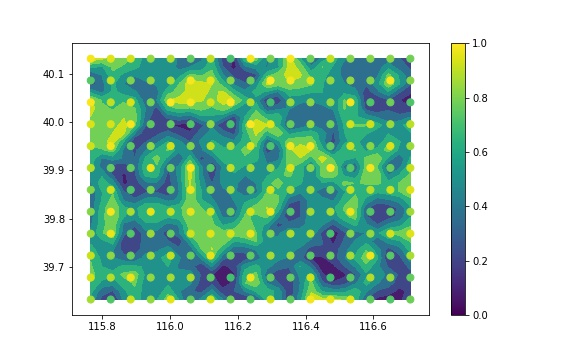
\includegraphics[width=\linewidth]{well_covered_meshgrid.jpg}
 		\caption{Buona Data Coverage}
 	\end{subfigure}\hfill
 	\begin{subfigure}[b]{0.5\linewidth}
 		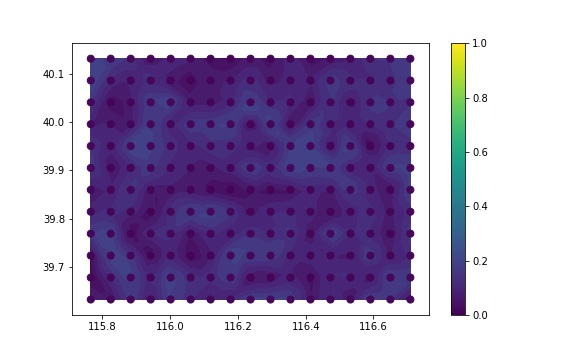
\includegraphics[width=\linewidth]{badly_covered_meshgrid.jpg}
 		\caption{Cattiva Data Coverage}
 	\end{subfigure}\hfill
 	\caption[Esempio di Data Coverage]{Esempi di Data Coverage su una griglia di locazioni}
 	\label{fig:coverage_examples}
 \end{figure}

\ \\ \\
 
 
La presente tesi ha come obiettivo quello di implementare una misura di copertura utilizzando un modello probabilistico che tenga conto della mobilità degli utenti che partecipano alla campagna.
Tale modello deve essere facilmente utilizzabile in scenari di raccolta dati differenti.
Al fine di misurare la Data Coverage, è stato analizzato ed esteso il data set GeoLife \cite{zheng1,zheng2,zheng3}.
Il data set offre tracciati GPS raccolti su base volontaria in un periodo temporale molto ampio; questo porta a problematiche di vario tipo: la campionatura dei punti GPS non è regolare e vi sono intere settimane nel nostro data set che mancano di dati significativi per la scarsa partecipazione degli utenti; nel corso della tesi tale data set è stato esteso, generando in questo modo Augmented Geolife, di cui daremo una descrizione approfondita nel Capitolo 3, dopo aver parlato del data set originale.

\section*{Obiettivi della Tesi}


La presente tesi ha due obiettivi principali:
\begin{enumerate}
	\item Analizzare ed estendere un data set di mobilità
	\item Sviluppare un modello di Data Coverage
\end{enumerate}

In merito al primo obiettivo la tesi ha permesso di ottenere un data set aumentato per la città di Pechino, contenente una quantità di dati sufficienti al prosieguo delle analisi.
In merito al secondo obiettivo, lo sviluppo del modello di Data Coverage e la sua applicazione a differenti scenari applicativi, ci ha permesso di ottenere delle mappe di probabilità di copertura dell'area oggetto della campagna di Crowdsensing.
Tali mappe ci possono aiutare a pianificare future campagne di acquisizione dati, e sono sufficientemente chiare da permettere una identificazione rapida ed efficace delle zone che risultano essere scoperte, zone per cui dovremo probabilmente prevedere campagne di raccolta ad hoc.

La misurazione della Data Coverage è di estrema importanza per una serie di motivi: oltre a permetterci di valutare in modo quantitativo l'efficacia di una campagna di crowdsensing, ci fornisce anche un modo per pianificare ulteriori meccanismi di raccolta dati che siano complementari al paradigma di MCS. Uno tra questi potrebbe essere l'utilizzo di droni da inviare su richiesta nelle zone scarsamente coperte, in modo da migliorarne il parametro di coverage.
Un altro dei vantaggi della misurazione della Data Coverage è quello di dare informazioni su quali siano le aree urbane scarsamente popolate o trafficate. Grazie alla visualizzazione grafica dei data set di probabilità ottenuti per i vari scenari, è possibile comprendere facilmente tali risultati sperimentali.

\section*{Metodologia e Risultati}

\subsection*{Metodologia usata}

Per raggiungere i nostri scopi ci siamo avvalsi di una serie di librerie software all'avanguardia nel campo della mobilità, dell'analisi dati e della visualizzazione di questi ultimi. Nella Sezione 1.3 presenteremo le librerie che ci hanno aiutati maggiormente nella nostra analisi. Tra di esse è sicuramente importante ricordare scikit-mobility \cite{pappalardo2019scikitmobility}, strumento grazie al quale abbiamo elaborato con semplicità ed efficacia i dati spaziali.
Nel corso della tesi abbiamo progettato e sviluppato processi simulativi per arricchire il data set Geolife con ulteriori traiettorie.
L'utilizzo di strumenti di visual analytics ci ha infine permesso di rappresentare le proprietà dei dati spaziali che abbiamo analizzato.

\subsection*{Risultati ottenuti}

Lo studio ci ha condotti allo sviluppo di opportune analitiche per misurare le proprietà del data set GeoLife, tra di esse citiamo il numero di utenti attivi in un determinato periodo temporale, i punti di partenza e di arrivo delle traiettorie degli utenti, i flussi di spostamenti sulla città di Pechino.

Abbiamo inoltre sviluppato un simulatore di tracce che, per mezzo di interpolazioni e calcoli di distanze, permette di generare serie temporali di traiettorie sintetiche con una certa precisione basandoci su punti di partenza e di arrivo.

Altro importante risultato ottenuto è l'implementazione di un modello di Data Coverage basato sulla probabilità di detour degli utenti. 

I risultati della applicazione del modello ai vari scenari sono presentati nel Capitolo 4 assieme a delle mappe di calore che ne riassumono graficamente il significato. La rappresentazione grafica ci mostra intere zone completamente scoperte per ciascuno dei tre scenari che abbiamo preso in esame, e ci invita a indagare soluzioni future atte a migliorare la Data Coverage nella zona che abbiamo preso come riferimento.
Di tali sviluppi futuri facciamo menzione nel Capitolo 5.
